\section{Approach}
\label{sec:approach}

In this section, we describe the model architecture used for our experiments
and propose our novel repetition reduction method, which is an extension to the basic model.
~\footnote{
All of the data and source code
can be downloaded from http://202.120.38.146/sumrep.}

In summarization task, the input (source document) and
output (summary) are both sequences of words.
Suppose the input and output are respectively represented as
$\textbf{x} = (x_{1},x_{2},...,x_{m})$ and 
$\textbf{y} = (y_{1}, y_{2},..., y_{n})$ ($m>n$),
the goal is to maximize the conditional probability
$p(\textbf{y}|\textbf{x})$:
\begin{equation}
p(\textbf{y} | \textbf{x}) \!=\! {\prod^n_{t} {p(y_{t} | y_{1}, y_{2},..., y_{t-1}, \textbf{x}})}
\end{equation}

Furthermore, we aim to generate summaries that are not only fluent 
and logically consistent with the source documents, but also with 
a small amount of repeatedness, which is natural in human written summaries.  

\subsection{Basic CNN seq2seq Model}
\label{sec:basic}
Our basic model is multi-layer convolutional seq2seq networks \citep{gehring2017convs2s} with attention mechanism
\footnote{\url{https://github.com/facebookresearch/fairseq-py}}, 
as illustrated in \figref{fig:basicModel}. 

\begin{figure}[th]
    \centering
    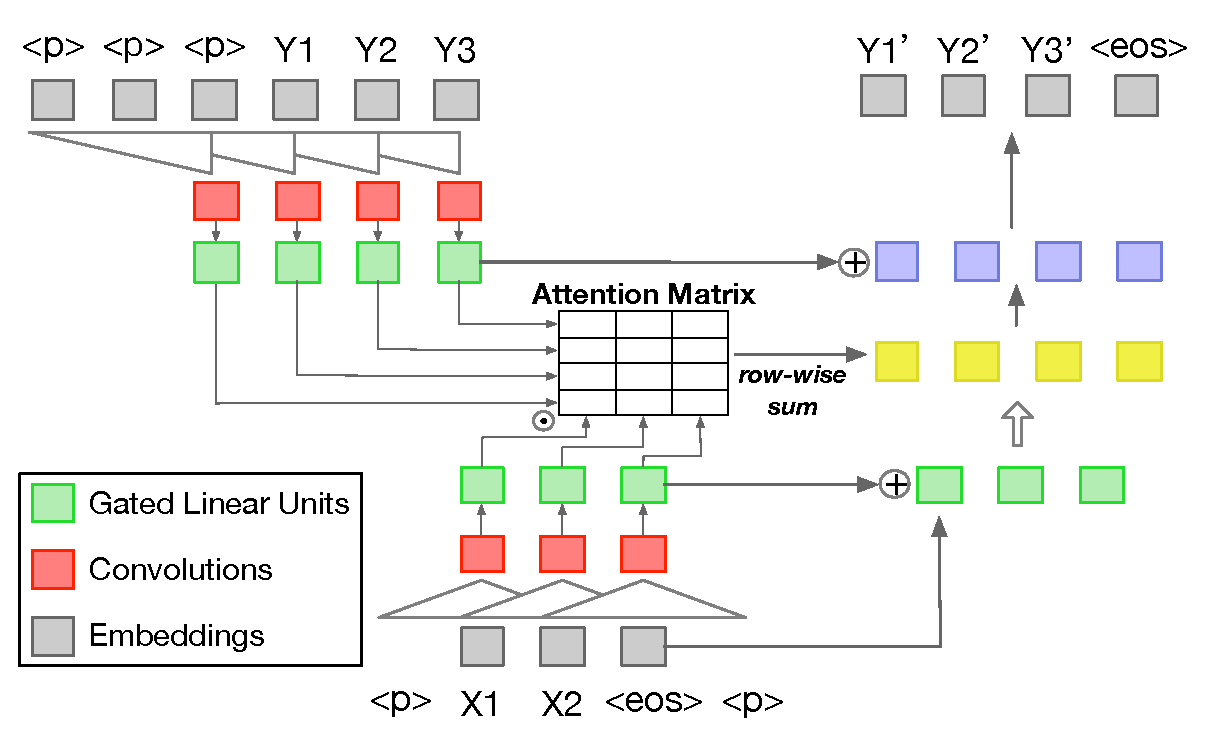
\includegraphics[width=0.7\linewidth]{cnn}
    \caption{Convolutional seq2seq model.}
    \label{fig:basicModel}
\end{figure}


For CNN seq2seq models, we combine word embeddings and position embeddings to obtain input $\mathbf{X} = (X_1,...,X_m)$ and output $\mathbf{Y}=(Y_1,...,Y_n)$. 
We denote $\mathbf { z } ^ { l } = \left( z _ { 1 } ^ { l } , \ldots , z _ { m     } ^ { l } \right)$ and $\mathbf { h } ^ { l } = \left( h _ { 1 } ^ { l } , \ldots , h _ { n } ^ { l } \right)$ 
respectively as convolutional output of the encoder and
decoder in the $l$-th layer.
Each element of the output generated by the decoder network is fed
back into the next layer of decoder network.
In each layer, GLU \citep{DauphinFAG17} and residual connections \citep{HeZRS16}
are used respectively as a non-linear gate and guarantee for sufficient depth of the network.  
\begin{equation}
    h _ { i } ^ { l } = GLU \left( W ^ { l } \left[ H _ {i-k/2 } ^ { l - 1 } , \ldots , H _ { i+k/2 } ^ { l - 1 } \right] + b _ { w } ^ { l } \right) + H _ { i } ^ { l - 1 }
\end{equation} 
where \textit{k} is kernel width. $W$ and $b$ are trainable parameters.

For each decoder layer, the multi-step attention integrates encoder information. 
We compute decoder state $d_{i}^{l}$ for attention via
\begin{align}
    d _ { i } ^ { l } &= W _ { d } ^ { l } h _ { i } ^ { l } + b _ { d } ^ { l } + Y _ { i } \\
    a _ { i j } ^ { l } &= \frac { \exp \left( d _ { i } ^ { l } \cdot z _ { j } ^ { u } \right) } { \sum _ { t = 1 } ^ { m } \exp \left( d _ { i } ^ { l } \cdot z _ { t } ^ { u } \right) } \label{eq:a} \\
    c _ { i } ^ { l } &= \sum _ { j = 1 } ^ { m } a _ { i j } ^ { l } \left( z _ { j } ^ { u } + X_j \right) \label{eq:c}\\
	H_i^l &= c _ { i } ^ { l } + h_i^l \label{eq:H}
\end{align}
where $d_{i}^{l}$ is decoder state, $z_{j}^{u}$ is the encoder state, 
$u$ is the last layer of encoder
and $a_{ij}$ is attention score.
The inner product between decoder state and encoder outputs is used 
to measure the affinity. 
The conditional input to the current 
decoder layer is a weighted sum of the encoder states and input representations.
We get $H^l_i$ by adding $c _ { i } ^ { l }$ to $h_{i}^{l}$, which forms the input for the next decoder layer or the final output.

Finally, we compute the probability distribution for the next word
using the top decoder output:
\begin{equation}
	p \left( y _ { i + 1 } | y _ { 1 } , \ldots , y _ { i } , \mathbf { x } \right) = \operatorname { softmax } \left( W _ { o } H _ { i } ^ { L } + b _ { o } \right)
\end{equation}

\subsection{Attention Filter Mechanism (ATTF)}
\label{sec:attf}

\begin{figure}[th]
	\centering
	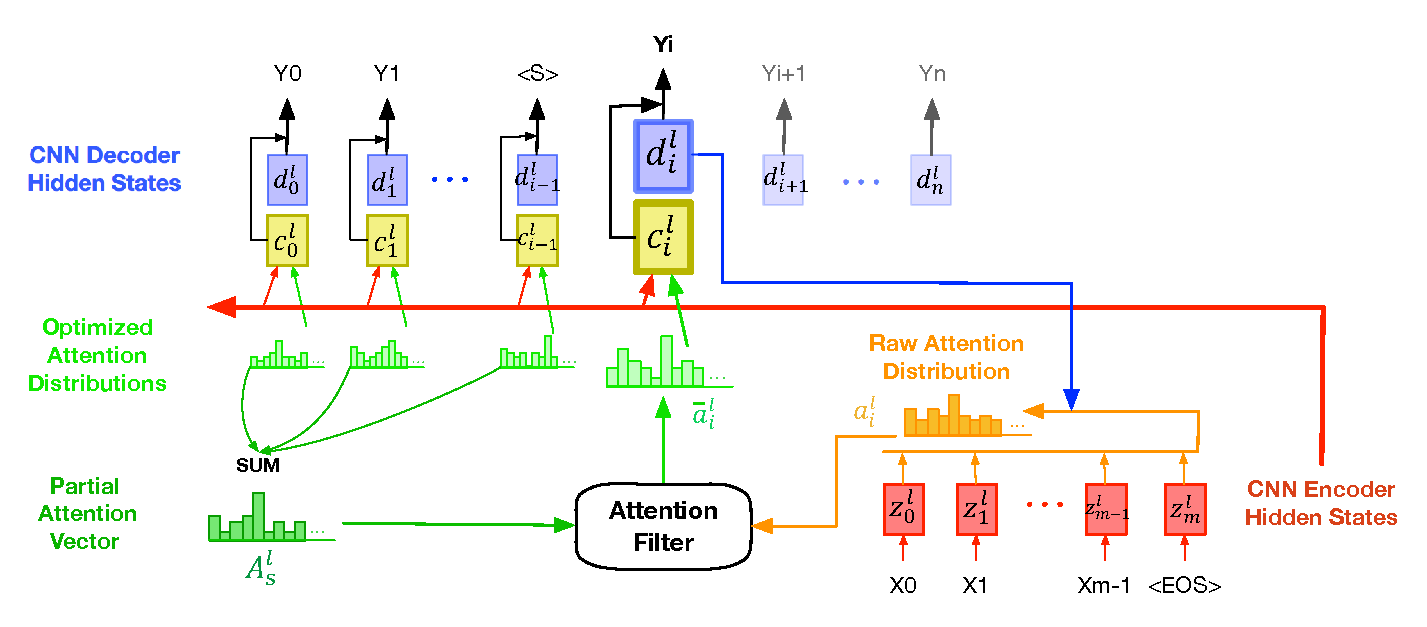
\epsfig{file=model.eps, width=0.9\columnwidth}
	\caption{Overview of Attention Filter Mechanism (ATTF)}
	\label{fig:model_main}
\end{figure}


\label{sec:attnf}
We propose an attention filter mechanism as a novel extension 
to the basic model,
which can record previously attended locations 
in the source document directly and generate summaries 
with a natural level of repeatedness. 
This method aims at relieving the repetition problem caused by 
decoders attending to the same POI in source document.

\subsubsection{Notations}
In this mechanism, both source document and summary are 
respectively split into segments by punctuations. 
For the convenience of description, 
we take ``{\em sections}'' as the segments in source document and ``{\em segments}'' as the segments in summary. 
We denote the punctuation marks as \verb#<S>#.
$\mathbf{u}=(u_{0},u_{1},...,u_{M})$ 
denotes the positions of \verb#<S># in source document and $\mathbf{v}=(v_{0},v_{1},...,v_{N})$ denotes the positions of \verb#<S># in summary.
Both $u_{0}$ and $v_{0}$ are $-1$.
Therefore, we can represent source document as $\mathbf{U}=(U_{1},U_{2},...,U_{M})$ and $\mathbf{V}=(V_{1},V_{2},...,V_{N})$ as summary.
$U_i$ is the $i$-th {\em section} and 
$V_i$ is $i$-th {\em segment}.
Both $U_i$ and $V_i$ are the sequence of 
tokens without punctuation tokens.

Let $D$ denote the number of tokens in the source document.
$a_i^l=(a_{i1}^l, a_{i2}^l,..., a_{ij}^l,..., a_{iD}^l)$ is a $D$-dimensional vector that records 
the attention scores in $l$-th layer of the $i$-th token in the summary over 
tokens in the source document.
We define \textit{segment attention vector} in the $l$-th layer as 
$A^{l}=(A_{0}^{l}, A_{1}^{l},..., A_{N}^{l})$.
For $s$-th \textit{segment} $V_s$, 
$A_s^l=(A^l_{s1}, A^l_{s2},...,A^l_{sD})$ 
is a vector representing 
segment attention distribution
over tokens in the source document.
$A^l_{sj}$ is the attention score between $V_s$ and $j$-th token in the source document.

\subsubsection{Description}
\label{sec:des}
To measure the relevance between $j$-th token of the source document 
and the $s$-th \textit{segment} $V_s$,
we sum up attention scores 
of each token in the $s$-th \textit{segment} over $j$-th token of the source document :

\begin{equation}
    A_{sj}^{l} = \sum_{i=v_{s-1}+1}^{v_{s}-1}a_{ij}^{l}
\end{equation}
We set $A_{0}^{l}$ as a zero vector, because nothing is attended before generating 
the first \textit{segment}. 


To find the most attended \textit{sections} of {\em segment} $V_s$, 
we sort the elements inside the filter vector, 
$A_{s}^{l}$, in descending order, 
and record the top $k$ elements' positions in 
the source document as: 
$\mathbf{p}=(p_{1},...,p_{k})$
where $k=v_{s}-v_{s-1}-1$. 
In the other words, 
$\mathbf{p}$ records the position of $k$ words most attended to $V_s$ in the source document.
$k$ is the same as the number of tokens in the $s$-th \textit{segment},
because each token in a \textit{segment} is aligned with at least one token in source document, according to the principle of the seq2seq model.
Thus, for the $s$-th \textit{segment}, 
we can find its most attended \textit{sections} by $\mathbf{p}$.
We locate the elements at $\mathbf{p}$ in the source document as well as
the \textit{sections} they belong to. 
For {\em section} $U_t$, we take the tokens that belong to $U_t$ and are located in the positions of $\mathbf{p}$ as $P_{U_{t}}$. 
If the size of $P_{U_{t}}$ is larger than
$\beta$, a predefined constant,
the \textit{section} $U_{t}$ is a POI of {\em segment} $V_{s}$,
which should not be attended to again. 
$\mathbb{U}_{s}$ denotes a set of all such POIs for $V_s$.
$\mathbb{U}_{0}$ is an empty set.

We construct two multi-hot vectors $g_{s}$ and $g'_{s}$ for each \textit{segment} $V_{s}$.
The dimensions of them are the number of tokens in source document, $D$, 
which are the same as the dimension of $A_{s}^{l}$. 
For $g_{s}$, we set elements on the position of tokens
belonging to sections in $\mathbb{U}_{s}$ to 0, and the elements on other
positions to 1. 
$g_{sj}$ is the $j$-th elements of $g_s$.
If $g_{sj}=0$, it means that the $j$-th token is attended by {\em segment} $V_s$ during the generation of $V_s$.
$g'_{sj}$ is $j$-th element of $g'_{s}$, which is the flipped version of $\prod \limits_{q=1}^{s}g_{qj}$. 
In the other words, $g'_{sj}$ is $1-\prod \limits_{q=1}^{s}g_{qj}$.
If $\prod \limits_{q=1}^{s}g_{qj}=0$ and $g'_{sj}=1$, it means that the $j$-th token of the source document has been attended before.
The filter on $a_{ij}^{l}$ in Equation (\ref{eq:a}) is given as:
\begin{equation} \label{eq:dis}
	\tilde{a}_{ij}^{l} = a_{ij}^{l}\prod_{q=1}^{s}g_{qj} + \min \limits_{A_{s}}\left(\frac{A_{sj}^{l}}{v_{s}-v_{s-1}-1}\right)g_{sj}'
\end{equation}
where 
$\tilde{a}_{ij}^l$ is the filtered attention score. 
$A_{sj}$ is the attention score between $j$-th token
of the source document and the $s$-th \textit{segment}. 
$g_{sj}$ and $g_{sj}'$ denote whether $j$-th token
of the source document has been attended.
We penalize the attention score of attended tokens in source document.
We take the minimum attention score between tokens in source document and summary 
(i.e. $\min \limits_{A_{s}}\left(\frac{A_{sj}^{l}}{v_{s}-v_{s-1}-1}\right)$ )
as the attention score between the $i$-th token in target 
and the attended tokens in the source.
Equation (\ref{eq:c}) now becomes
~\footnote{After Equation (\ref{eq:dis}), 
	an alternative way to get $c^l_i$ is to use the re-normalized filtered attention scores $\tilde{a}_{ij}^l$. We re-normalize the filtered attention scores by $\tilde{\textbf{a}}_i^l=softmax(\tilde{a}_{i}^l)$ where $\tilde{a}_{i}^l=(\tilde{a}_{i1}^l, \tilde{a}_{i2}^l,......,\tilde{a}_{iD}^l)$. 
	Then, Equation (10) becomes 
	$\tilde{c} _ { i } ^ { l } = \sum _ { j = 1 } ^ { m } \tilde{\textbf{a}}_{ij}^{l} \left( z _ { j } ^ { u } + X_j \right)$.}:
\begin{equation} 
	\label{eq: ccc}
    \tilde{c} _ { i } ^ { l } = \sum _ { j = 1 } ^ { m } \tilde{a}_{ij}^{l} \left( z _ { j } ^ { u } + X_j \right)
\end{equation}


By using segment-wise attention and revising attention scores of attended POIs directly,
our model optimizes the
attention distribution between the encoder states and decoder states in such a way that
the alignment relationship between source document and summary is enhanced, 
and noise for attention from encoder outputs is reduced. 
As shown in \tabref{tab:attn_exp}, the segments in the example are separated by punctuation.
For the basic CNN model, the 2nd and 3rd sentence repeatedly attend to 
the 5th segment in source document.
After applying ATTF model, 
the attention scores of the 3rd and 5th segment in source document are penalized 
during generating words in the 3rd sentence of ATTF.
The last sentence of the summary generated by ATTF attend to the $7$-th segment in source.

\begin{table}[th!]
\begin{center}
\caption{\label{tab:attn_exp} Summary generated by the basic CNN model and ATTF model. The {\em segments} of summary use the same color as their attended {\em section} in the source document.}
\begin{tabular}{rl}
\toprule[1pt] 
\multicolumn{2}{c}{\bf Source document} \\
\hline
\multicolumn{2}{c}{\tabincell{l}{(1)justin timberlake and jessica biel, (2)welcome to parenthood. 
	   (3)\textcolor{red}{the celebrity couple} \\
           \textcolor{red}{announced the arrival of their son,} 
           (4)... (5) \textcolor{blue}{the couple announced the pregnancy in} \\
           	\textcolor{blue}{january,} (6)... (7)\textcolor{brown}{it is the first baby for both .} }} \\
\cmidrule[1pt]{1-2} 
\bf Basic CNN model (CNN) &
\tabincell{l}{(1)\textcolor{red}{the couple announced the the arrival of their son.} \\
	(2)\textcolor{blue}{the couple announced the pregnancy in january.} \\ 
	(3)\textcolor{blue}{the couple announced the pregnancy in january.}}  \\
\hline 
  \bf ATTF (our)
& \tabincell{l}{(1)\textcolor{red}{the couple announced the arrival of their son.} \\
	            (2)\textcolor{blue}{the couple announced the pregnancy in january.} \\
	            (3)\textcolor{brown}{it is the first baby for both.}} \\
\bottomrule[1pt]
\end{tabular}
\end{center}
\end{table}
The attention filter mechanism helps avoid repeatedly attending to the same POIs, and therefore avoid repetition in summary generation.


\subsection{Sentence-level Backtracking Decoder (SBD)}
\label{sec:sbd}

To tackle repeated sentences or phrases in the source (\exref{ex:repeatsrc}), 
we propose a sentence-level backtracking decoder.

\begin{figure}[th]
    \centering
    \includegraphics[width=0.7\linewidth]{SBD}
    \caption{Backtracking in Beam Search ($b=3$). 
	    This figure shows the progress of generating summary at test. The circles denote the
		candidate words (choices) in vocabulary, 
		which are sorted by the probability of being selected in
		descending order. Each circle at level $l$ has $N$ choices 
		at level $l+1$. $N$ is the number of words in vocabulary. 
		The number in circles is the order of these choices according to the
		probability. The generation order is from level 1 (top) to level 3 (bottom).}
    \label{fig:beam}
\end{figure}

At test time, we prevent the decoder from generating identical or
very similar sentences more than once via backtracking. 
An intuitive solution is to backtrack the generation process to the beginning
of the repeated segment, and regenerate it by following the second best choice
in the beam. We call this simple approach \textbf{SBD-b1}.
However, this is sub-optimal
because the parents of the current top $b$ choices may not include all the top $b$ choices at the
parent level. Here $b$ is the beam size. As shown in \figref{fig:beam}, suppose that level 3 is the
beginning of the repeated segment, the first choices at level 1 and 2 are excluded by beam search. 

An alternative approach (\textbf{SBD-b2}) backtracks all the way until the current
top $b$ choices all share the same prefix token sequence. This means
that the current best choices in the beam reach some consensus that
the generated prefix summary is good and should be retained. 
While this algorithm backtracks further and may
include better choices, it does not completely solve the problem of SBD-b1. 
As shown in \figref{fig:beam}, 
suppose that level 3 is the beginning of the repeated segment and the second choice in
level 1 is the only prefix token sequence of top $b$ choices in level 2, the first and third choices at
level 1 are excluded by beam search after generating words based on the second choice in level 1.

\begin{table}[th!]
\begin{center}
\caption{\label{tab:sbd_exp} Summary generated by basic CNN model with different backtracking methods.}
\begin{tabular}{rl}
\toprule[1pt]
\multicolumn{2}{c}{\bf Source document} \\
\hline
\multicolumn{2}{c}{\tabincell{l}{
justin timberlake and jessica biel , welcome to parenthood . the celebrity couple announced \\
the arrival of their son , silas randall timberlake ,... `` silas was the middle name of \\
timberlake 's maternal grandfather bill bomar , who died in 2012 ,... the couple announced \\
the pregnancy in january , with an instagram post . it is the first baby for both .
}} \\
\toprule[1pt]
\bf Basic CNN model (CNN)
& \tabincell{l}{
				the couple announced the arrival of their son. \\
			    the couple announced the pregnancy in january. \\
				\textit{the couple announced the pregnancy in january. (repeated segment)} \\
				} \\
\hline 
\bf CNN+TRI
& \tabincell{l}{
	the couple announced the arrival of their son. \\
	\underline{silas randall timberlake , who died in 2012.} \\
} \\
\hline
\bf CNN+SBD-b1
& \tabincell{l}{
				the couple announced the arrival of their son. \\
				the couple announced the pregnancy in january. \\
				\underline{silas was the middle name of timberlake 's maternal grandfather.} \\
				} \\
\hline
\bf CNN+SBD-b2
& \tabincell{l}{
				the couple announced the arrival of their son. \\
				\underline{silas randall timberlake , died in 2012.} \\
				} \\
\hline
\bf CNN+SBD
& \tabincell{l}{
				the couple announced the arrival of their son. \\
                they announced the pregnancy in january, with an instagram post. \\
				} \\
\bottomrule[1pt]
\end{tabular}
\end{center}
\end{table}

Our best approach (\textbf{SBD}) backtracks to the beginning of the whole summary
and regenerates all the choices in the beam up to the point before
the repeated segment. That way, all the best choices are known to the
algorithm and we can make an optimal choice after excluding the first word
of the previously repeated segment. 
As shown in \tabref{tab:sbd_exp},
SBD-b1 and SBD-b2 backtrack the generator process
to ``january.'' and ``son.'' respectively.
The summaries generated by SBD-b1 and SBD-b2 
are incoherent and inconsistent with the source document.
Our best approach (SBD) will save the sequence before repeated segment, i.e., 
`\textit{
the couple announced the arrival of their son.
the couple announced the pregnancy in january.}
'
and backtrack to the beginning of the summary and regenerate the summary. 
When the saved sequence appears in the beam, we remove the first word (``the'') in 
repeated segment from the choices vocabulary. 
Compared with SBD-b1 and SBD-b2, SBD generates more fluent and coherent summaries.


To determine whether two sentences, 
$p$ and $q$, are similar, we define a boolean function as:
\begin{equation}\label{eq:s}
	sim(p,q) = 
	\begin{cases}
		   1 &\mbox{if $o(p,q) > n\text{ OR }o(p,q) > \frac{1}{2}\cdot l$}\\
		   0 &\mbox{others}
   \end{cases}
\end{equation}
where $o(p,q)$ denotes the length of 
the longest common substring (LCS) between $p$ and $q$, 
$l$ is the minimum of the lengths of $p$ and $q$, and $n$ is a constant. 
$sim(p,q)=1$ means the two sentences are similar.

This method cooperates with ATTF in 
reducing repetition caused by the noises in dataset.
Compared with \textbf{TRI},  SBD does not interrupt the beam search process in the middle of a sentence, hence significantly reducing related grammatical and factual errors. 
As shown in \tabref{tab:sbd_exp}, 
the summary generated by SBD is grammatical and factual. 
Besides, SBD is capable of producing a more informative summary since it yields more chances to other candidate sentences.
